\scalebox{1}{\begin{tikzpicture}
\node[inner sep=0pt] (peak) at (0,0)
    {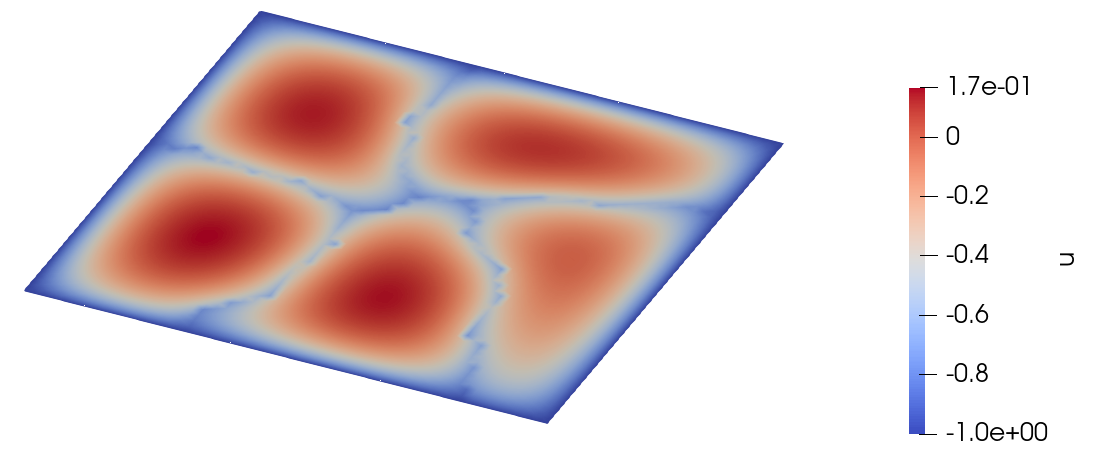
\includegraphics[width=0.9\textwidth]{images/base1.png}};
\node[inner sep=0pt] (peak1) at (1.5,-3.8)
    {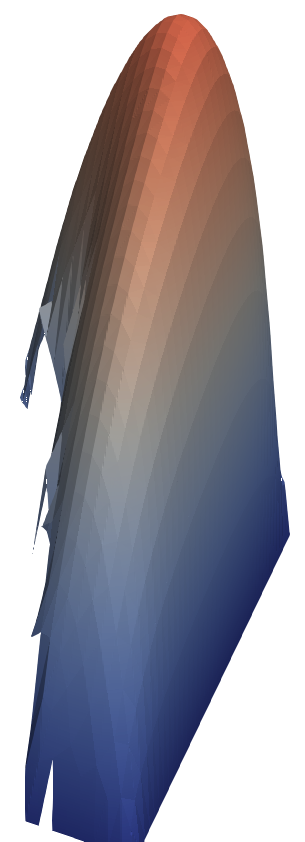
\includegraphics[width=.15\textwidth,height=0.3\textwidth]{images/peak1.png}};
\draw[->,thick] (0.2,-0.6) -- (peak1.north) node[midway,fill=white] {\footnotesize $T_1(u^0)$};
\node[inner sep=0pt] (peak2) at (-2.5,-3.8)
    {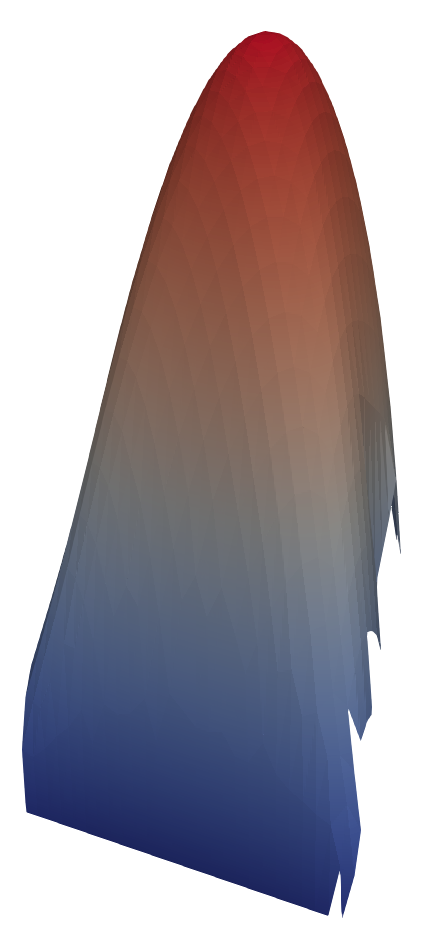
\includegraphics[width=.2\textwidth,height=0.34\textwidth]{images/peak2.png}};
\draw[->,thick] (-1.4,-0.6) -- (-2.2,-2.3)node[midway,fill=white] {\footnotesize $T_2(u^0)$};
\end{tikzpicture}}